%!TeX root = Chapter_Data
\documentclass[../../CompleteThesis/Complete_1stDraft]{subfiles}

\begin{document}

\section[Selection][Selection]{Selection of Data}
\label{Sec:Data_Selection}
\subsection[AWI B-cores]{AWI B-cores: Core B23}
\label{Subsec:Data_Selection_Bcores}


\begin{figure}[h]
	\centering
	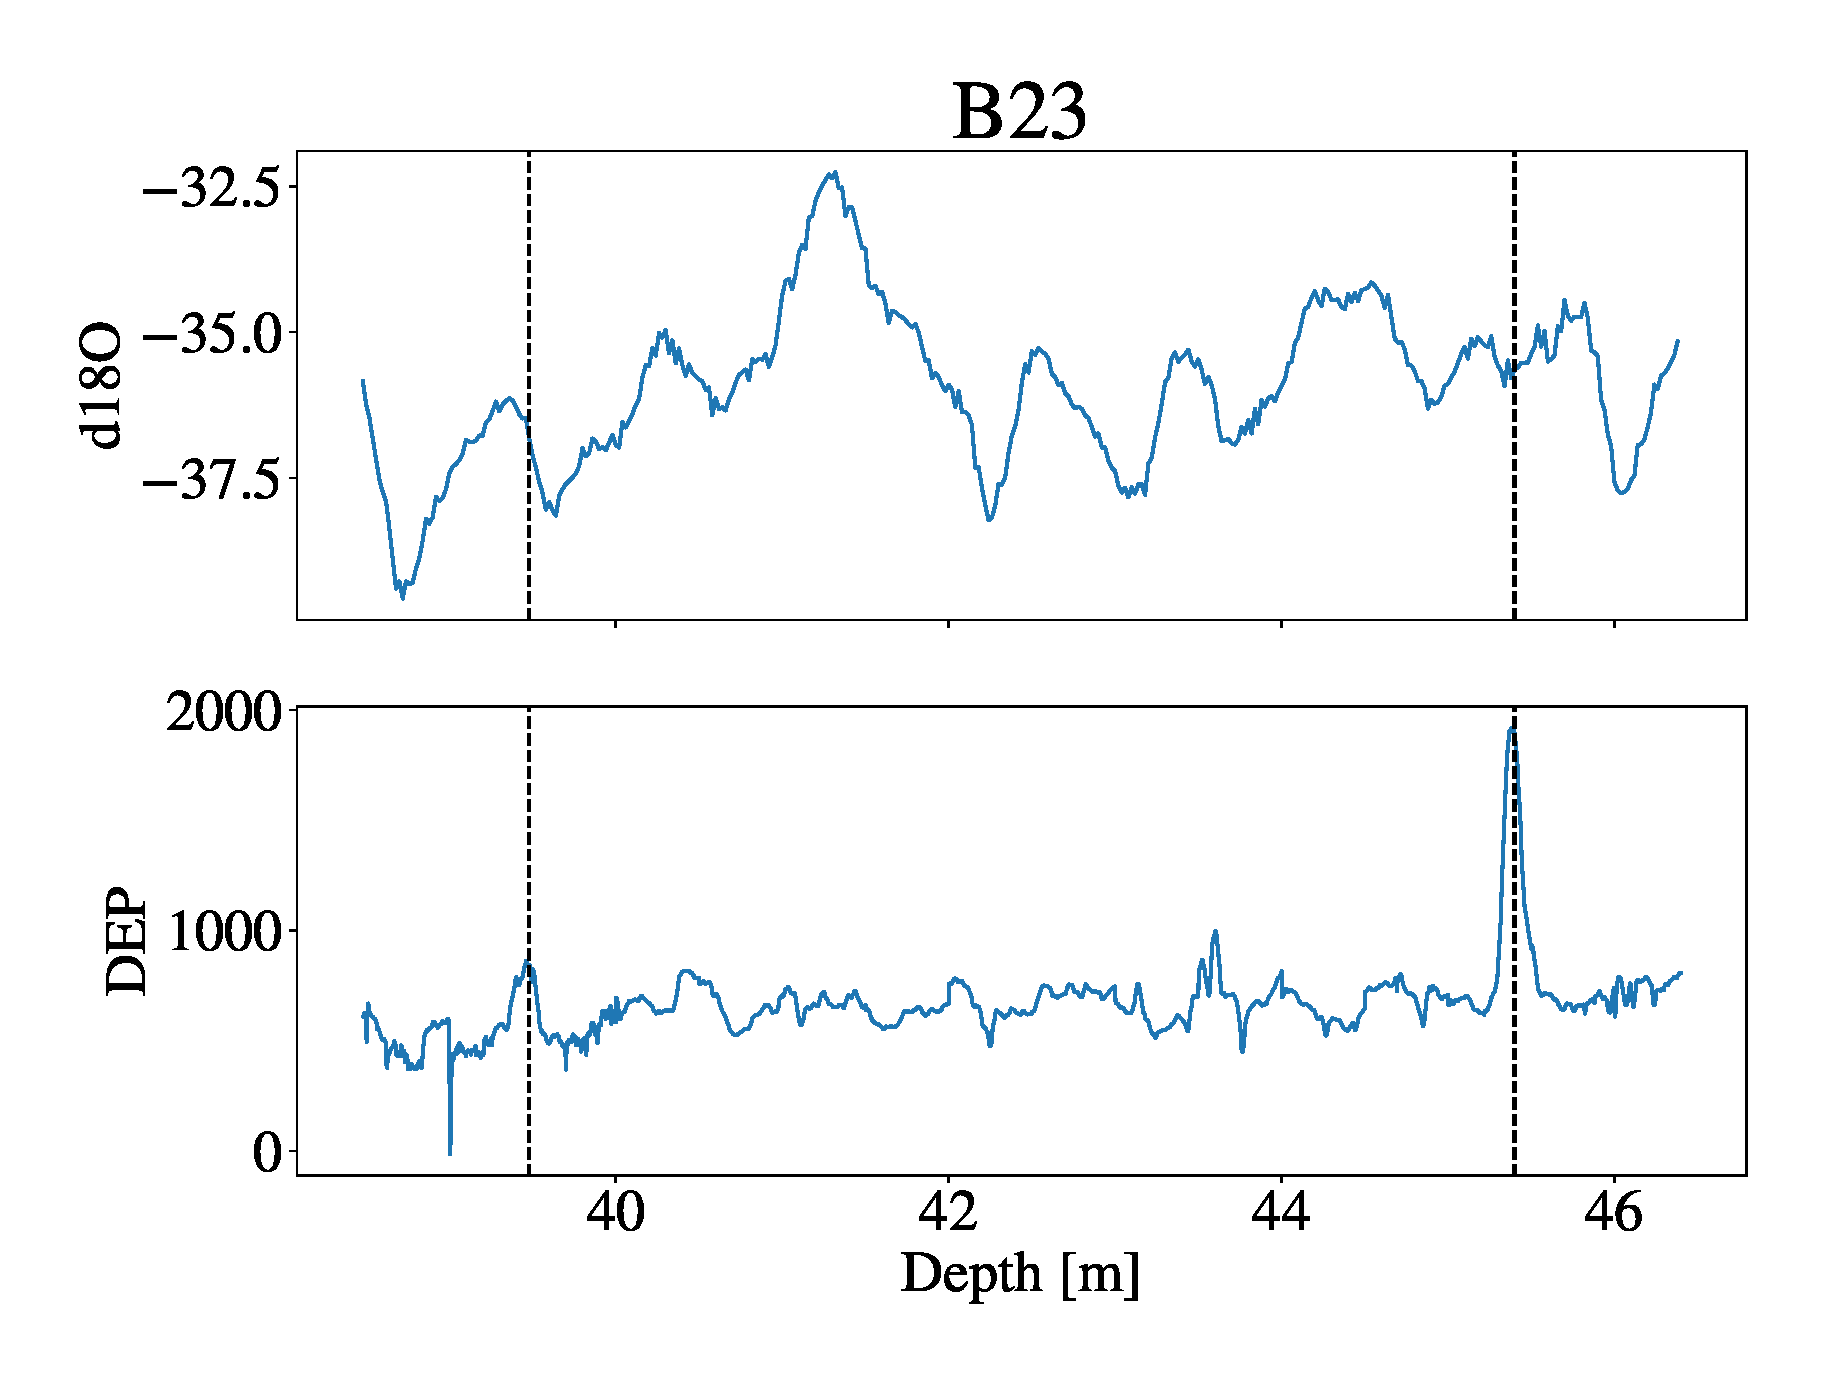
\includegraphics[width=0.8\textwidth]{Core_LT_B23.eps}
	\caption[]{}
	\label{fig:Core_LT_B23}
\end{figure}

\begin{figure}[h]
	\centering
	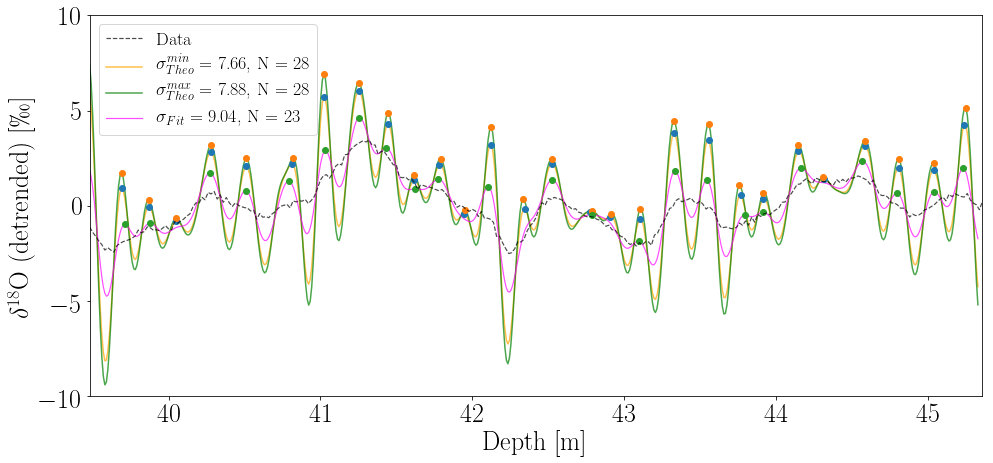
\includegraphics[width=0.8\textwidth]{B23_TheoDiffLens33Theo.png}
	\caption[]{}
	\label{fig:B23_BD_Theo}
\end{figure}

\begin{figure}[h]
	\centering
	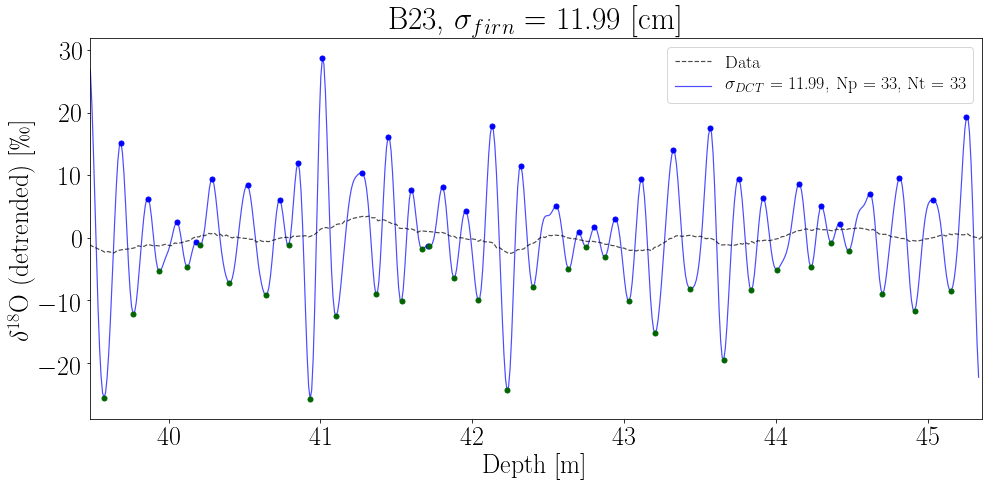
\includegraphics[width=0.8\textwidth]{B23_TheoDiffLens33Opt_only.png}
	\caption[]{}
	\label{fig:B23_BD_OptOnly}
\end{figure}

\begin{figure}[h]
	\centering
	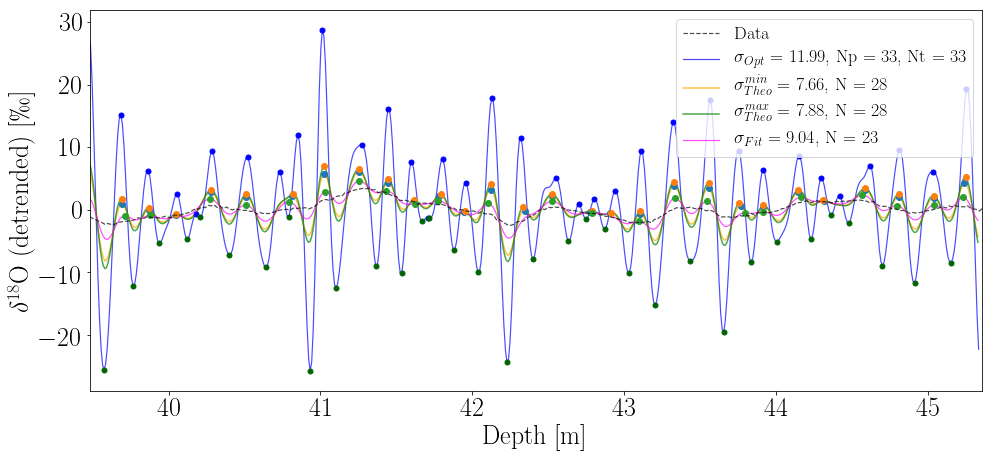
\includegraphics[width=0.8\textwidth]{B23_TheoDiffLens33OptBig.png}
	\caption[]{}
	\label{fig:B23_BD_OptBig}
\end{figure}


\subsection[Crete Area][Crete Area]{Crete and Surrounding Alphabet Cores: Site A}
\label{Subsec:Data_Selection_Alhabet}

\begin{figure}[h]
	\centering
	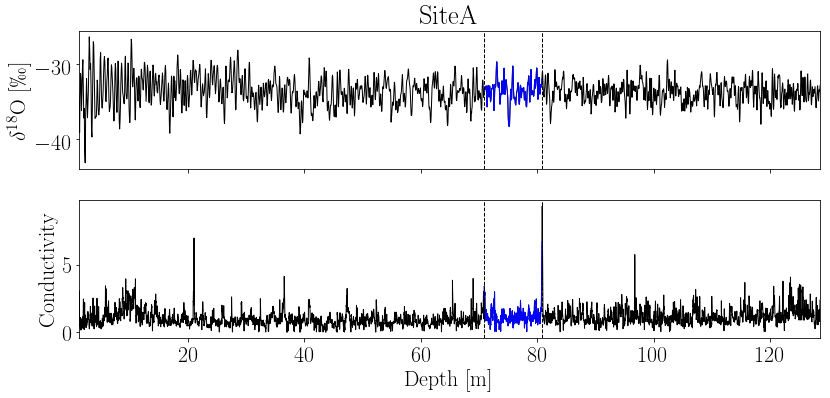
\includegraphics[width=\textwidth]{SiteA_ECM_d18O_full.png}
	\caption[]{}
	\label{fig:SiteA__ECM_d18O_full.png}
\end{figure}

\begin{figure}[h]
	\centering
	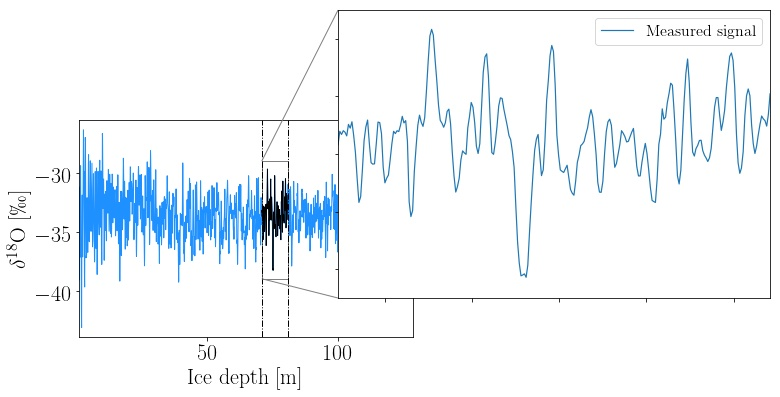
\includegraphics[width=\textwidth]{SiteA_d18OInsert.jpg}
	\caption[]{}
	\label{fig:SiteA_d18OInsert}
\end{figure}

\begin{figure}[h]
	\centering
	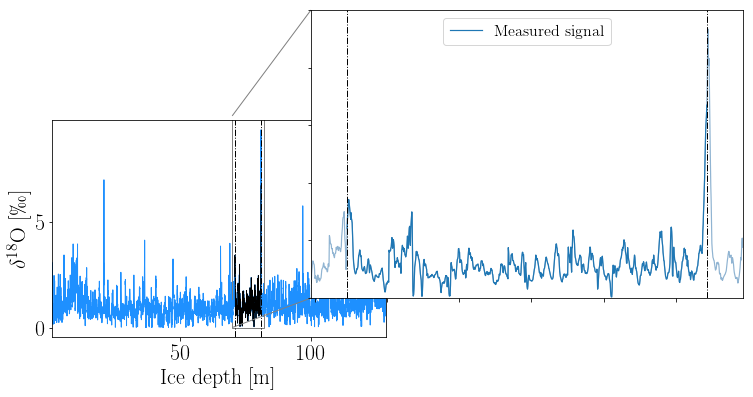
\includegraphics[width=\textwidth]{SiteA_ECMInsert.png}
	\caption[]{}
	\label{fig:SiteA_ECMInsert}
\end{figure}

\begin{figure}[h]
	\centering
	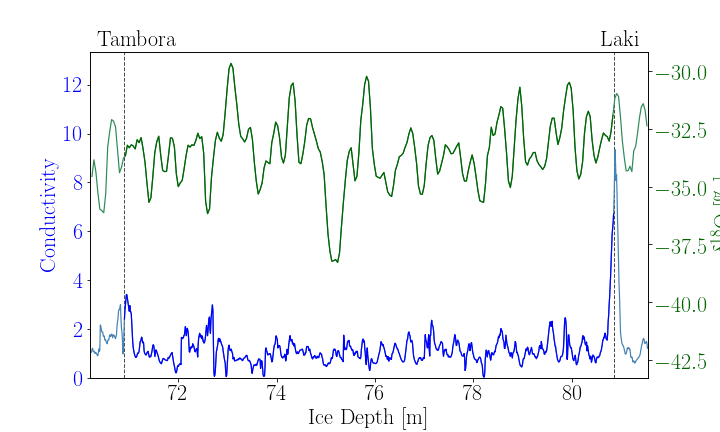
\includegraphics[width=\textwidth]{SiteA_ECMd18O_combo.png}
	\caption[]{}
	\label{fig:SiteA_ECMd18O_combo}
\end{figure}

\section[Data Specifications][Data Specifications]{Data Specifications}
\label{Sec:Data_Specifications}


\end{document}